\documentclass[a4paper,12pt]{article}

\usepackage{graphicx}	
\usepackage{pdfpages}
\usepackage{booktabs}	
\usepackage{csquotes}
\usepackage{hyperref}
\usepackage{multirow}
\usepackage[style=authoryear-ibid,backend=biber]{biblatex}
\addbibresource{mybib.bib}

\newcommand\addrow[2]{#1 &#2\\ }

\newcommand\addheading[2]{#1 &#2\\ \hline}
\newcommand\tabularhead{\begin{tabular}{lp{8cm}}
\hline
}

\newcommand\addmulrow[2]{ \begin{minipage}[t][][t]{2.5cm}#1\end{minipage}% 
   &\begin{minipage}[t][][t]{8cm}
    \begin{enumerate} #2   \end{enumerate}
    \end{minipage}\\ }

\newenvironment{usecase}{\tabularhead}
{\hline\end{tabular}}
\begin{document}

\begin{titlepage}

\newcommand{\HRule}{\rule{\linewidth}{0.5mm}}

\title {Carers Scheduling Prototype Software Application}

\author{John O'Grady}
\date{April 2017}

\maketitle

\thispagestyle{empty}

\begin{center}
\HRule \\[0.4cm]
\textsc{\large Submitted in part fulfilment
 \\for the Higher Diploma in Computing
\\School of Informatics and Engineering,
\\Institute of Technology Blanchardstown,
\\Dublin, Ireland
} 
\end{center}

\HRule \\[2cm]

%----------------------------------------------------------------------------------------
%	AUTHOR SECTION
%----------------------------------------------------------------------------------------

\begin{minipage}{0.4\textwidth}
\begin{flushleft} \large
\emph{Author:}\\
 \textsc{John O'Grady} 
\end{flushleft}
\end{minipage}
~
\begin{minipage}{0.4\textwidth}
\begin{flushright} \large
\emph{Supervisor:} \\
\textsc{Dr. Matt Smith} 
\end{flushright}
\end{minipage}\\[2cm]

\begin{center}

\includegraphics{itb_logo.jpg}
\end{center}

\end{titlepage}
\pagenumbering{arabic}

%----------------------------------------------------------------------------------------
%	Brief overview of project, aims, methodology and approach taken
%----------------------------------------------------------------------------------------
\section*{Abstract}

This project is concerned with requirements gathering, planning and delivery of a prototype rostering and scheduling software application for the Irish Wheelchair Association (IWA), a large non profit service provider which needs a new organisation wide software process to manage the planning of care appointments for people with disabilities. This project begins by setting the organisational context for the planned new software initiative. Next, it progresses to examine the body of current academic research in software delivery to provide a brief synthesis of best practice in the planning, implementation and deployment of modern software applications.

Based on this research, this author selects the Systems Development Life Cycle (SDLC) methodology as an appropriate toolset to determine the requirements of IWA for a new rostering and scheduling solution which the organisation plans to deploy to its 1,500 Personal Assistants. Having gathered the requirements, the project progresses to define the organisational context for the software deployment.

Using the SDLC methodology the author, who is responsible for leading the Information Technology function at IWA, works collaboratively with key project stakeholders across the organisation to define a broad functional requirement specification and produces various key design artefacts.

As the development work on the project progresses, a suite of SDLC mandated project management documents are iteratively refined and finalised. A high level test plan is developed and implemented to ensure code quality and alignment with user expectations and requirements.

Finally, in conclusion, the author offers some insights from his experience of the software planning and development process together with consideration of some areas for further investigation and ongoing improvement of the prototype which are outside the scope of the initial project build.

\pagebreak
\tableofcontents
\pagebreak------------------------------------------------
\begin{samepage}
\section{Introduction}

This project examines the requirements for a prototype Rostering and Scheduling solution for which the ultimate client, the Irish Wheelchair Association (IWA) has a real world business requirement. It is envisaged that the finished software deliverable at the conclusion of this project will not be a fully enterprise ready software solution but rather the project deliverable will be employed as a prototype for user acceptance testing by representative end users.  This software development process will be used to examine and further refine IWA's existing assumptions in relation to the imminent deployment of a critical real life deployment whose successful implementation is considered to be fundamental to the competitive position of the IWA. 

The scope of this project is to establish the detailed software functionality requirements for the new application and to utilise this information to deliver a prototype software solution for evaluation purposes which will cover the primary use cases and functional requirements identified. This will enable end users to test, assess and give feedback on the prototype and it is envisaged that this process will be constructive in mitigating the risk of any significant functionality components being omitted from the final production system or the usability of the ultimate solution not meeting user requirements in full. 

Following this iterative process, it is planned to document a more comprehensive set of final functional requirements for the production deliverable will fundamentally underpin a competitive tender exercise and vendor engagement through which IWA will select, configure and implement a live rostering and scheduling solution for its 1,500 Personal Assistants across Ireland.

\pagebreak
\section{Organisational Context}
\subsection {History of Irish Wheelchair Association}
The Irish Wheelchair Association (IWA) is a vibrant  independent organisation which was founded in 1960 by a group of people with disabilities. IWA is governed by a Board of Directors elected from its 20,000 membership base. It is the largest provider of Assisted Living Services in the Ireland, employing over 2,600 employees and delivering over 2 million hours of service annually. It is substantially funded by the Irish Government, primarily through the Health Service Executive, from whom it receives funding as a Section 39 agency under the Health Act 2004, although it also receives funding from various other statutory and non statutory sources and raises funds directly from the general public. A challenge which is directly pertinent to the planned software project is that IWA's funding revenue streams are primarily remitted in respect of service level agreements for the delivery of front line services and it receives no direct funding for Information Technology or indeed other Shared Services activities.

During the recent economic downturn and its impact on the public finances, IWA, like many non service providers, has had seen the government apply substantial cumulative funding cuts between 2008 and 2014. Against this backdrop IWA has managed to maintain and in some cases expand its level of service activity through pursuing internal efficiencies and implementing a series of pay reductions which have been agreed with its workforce but maintaining service delivery in the face of significant funding reductions has progressively diminished the financial reserves that the Association holds. 

These funding reductions have also significantly impacted on the state of IWA's Information Technology infrastructure which is now in need of attention following a sustained pattern of historic under investment. However, the organisation's strategic plan for the years 2017 to 2010 now views Information Technology initiatives as a core enabler of driving overall efficiency and value for money in its model of service delivery, on the strict understanding that approval of all capital investment decisions must be clearly linked to a defined and fully costed business case which will deliver an identifiable and measurable return on investment in net financial terms to the organisation. 

IWA has been at the forefront of developing person centred  service provision in Ireland, based on international best practice, and IWA is now somewhat unique among large charities in Ireland in that it remains wholly owned by, and accountable to its 20,000 members who made up of people with disabilities, active volunteers and other IWA supporters. In all areas of its activities, IWA advocates for independence and quality of life for all people with disabilities in Ireland. In this regard, the stated mission of IWA has recently been updated in its new Strategic Plan for 2017-2020 as follows:
\begin{displayquote}
Irish Wheelchair Association  has a vision of an Ireland where people with disabilities enjoy equal rights, choices and opportunities in how they live their lives, and where our country is a model worldwide for a truly inclusive society.
\end{displayquote}

In addition to Assisted Living Service, which is IWA's largest service employing 1,700 of IWA's 2,600 strong workforce, IWA provides a range of other services including a network of 57 community based Resource and Outreach Centres, respite services, driving tuition and a variety of member led youth and local branch projects. IWA Sport is a subsidiary division of IWA which is a recognised National Governing Body of Sport by the Irish Sports Council and IWA operates a network of volunteer led Sports clubs throughout Ireland which are an vibrant component of Ireland's Paralympic  movement, particularly with regard to the development of young disabled athletes.
IWA also has developed specialist teams in the specialist areas of Accessibility, Housing and Transport where it is widely acknowledged as an expert in providing expertise and advocacy in ensuring public and private developments are configured to meet the needs of people with disabilities.
\subsection {Overview of Assisted Living Service}
IWA's Assisted Living Service (ALS)  provides significant individual supports to people with disabilities which are tailored to the needs and wishes of the each person to enable them to live independently. IWA, with funding support from the Health Service Executive, provides a Personal Assistant (PA) to assist with tasks that the person with a disability might find difficult or impossible to do in their daily lives. Originating in the international Independent Living movement, which postulates that people with disabilities are best placed to make determinations on their own needs, IWA's ALS provides support to individuals in their homes and communities facilitating community participation, access to education, employment and improved quality of life. 

The ALS model of service delivery comes in two main strands
\begin{itemize}
\item  \textbf {Self-directed or leader-managed package. }In a self-directed or leader-managed package, the person with the disability acts as the leader or service manager for IWA. This involves recruiting their own personal assistants, organising their weekly rosters, returning their timesheets, arranging holiday cover, etc. The leader can consult the service coordinator when necessary.
\item \textbf {Supported package.} In the supported package, the service coordinator takes responsibility for some or all of the management, delivery and operation of the service.
\end{itemize} 

\subsection {Current Scheduling Process}
IWA does not currently have a unified scheduling, rostering and time attendance system in place across all of its ALS locations. A custom static (non calendarised) solution for roster and timetable planning functionality has been developed on its Microsoft Dynamics CRM environment and is currently in use across all IWA offices and a calendar based extension of this is currently in a pilot phase in a small number of IWA locations.  It is likely that IWA will migrate management of schedules and rosters to the new Rostering and Scheduling  platform however it should be noted that IWA does envisage continuing to use Dynamics CRM for other a variety of other key service management functions such as on-boarding service users, employee recruitment, risk assessments, evaluations and logging contact and activity information with employees and service users. 

While Microsocft Dynamics CRM has provided some basic functionality in relation to static rosters to date, in the absence of a fully calendarised roster solution across all IWA offices, local teams in IWA have developed a variety of long-standing and ad-hoc local solutions to managing planning rosters, all of which IWA wishes to discontinue in favour of the proposed new solution. 

The current IWA process for capturing  time and attendance information for payroll and billing purposes involves each PAs completing paper timesheets which are progressively signed off by the service user or a family member throughout the month at each service visit. 

At the end of the payroll month, the timesheets are delivered to the local coordinator at the local IWA office and are then data entered into the Focal-Point system. These timesheets are initially entered as ‘pending approval’ by an ALS Administrator within the system and routed to the ALS Coordinator for the service for approval. The coordinator reviews the timesheet against the expected visits and service budget and approves or amends the timesheet.

Once the Focal-point process is complete, an export of the approved timesheet data is taken from Focal Point and used to feed the Mega pay payroll system. The Mega pay application in turn feeds the Access Accounts system for invoicing/billing purposes. 
In the context of implementing a new rostering and time attendance system, IWA wishes to cease using Focal-point for the capture of Time and Attendance information and approval of same in favour of the new rostering and scheduling system directly managing the capturing and approval of time and attendance data which can then be exported directly to Access Accounts for billing purposes and Megapay for payroll processing.

\subsection {Overview of Organisational  Impacts}
%----------------------------------------------------------------------------------------
%	Background to work of IWA and context in which app will be used
%       Reference and link to live tender and explanation of tender approach
%       Description of service and roles who will use the live applciation
%	Definition and scope of prototype application
%----------------------------------------------------------------------------------------
The casual reader of the preceding section will quickly appreciate the inherent inefficiencies of the current paper centric process in an organisation of the size of IWA. Indeed, IWA employs a service management cohort of 26 Service Coordinators, 8 Service Support Officers and 20 Administrators across 15 ALS offices around Ireland and it has been estimated that across these employee groups, approximately 25\% of their working time is spent managing rostering and scheduling functions in relation to the ALS service to ensure all service visits are covered and a further 25\% of their time is currently consumed in manual data entry and approval tasks in relation to timesheet and payroll information. 

This inefficient process has a direct impact on IWA's cost base but also has an opportunity cost impact by limiting the available time of Service Coordinators to spend on other essential functions such as planning, evaluation, training and supervision activities. In this context, it should be noted that each IWA Service Coordinator is responsible for managing a large number (between 50-100 per Coordinator) of service packages for individual service users and each also supervise a similar number of Personal Assistants for whom the Service Coordinator acts as line manager. This also has an impact on the ratio of required back office personnel to service delivery hours and due to the somewhat manual rostering and scheduling process currently being operated,  IWA's service coordination and administration costs per service delivery hour are somewhat higher than some of its competitors, placing it at a competitive disadvantage, particularly in comparison to some of the private sector commercial operators who have recently entered the Irish homecare market and who in many cases currently have more sophisticated techological solutions in place to handle this key internal process. Note the scope of the project is defined in more detail in 

\subsection {Procurement and Tendering Approach}
IWA has recently launched the first phase of the competitive tender process for its new rostering and scheduling solution through the Office of Government Procurement's E-Tender's website which is available at \href{https://irl.eu-supply.com/app/rfq/publicpurchase_frameset.asp?PID=110399&B=ETENDERS_SIMPLE&PS=1&PP=ctm/Supplier/publictenders}{this link}
The first stage of the procurement process requires prospective vendors to complete a short pre-qualification questionnaire which provides an opportunity for vendors to demonstrate the capabilities of their software platform against the high level requirements summarised in the preceding section, as well as providing an overview of their organisational capability and customer references where they have already deployed their solution in a similar usage context.  
Following assessment of the pre-qualification questionnaires, IWA will shortlist a small number of interested vendors for the second phase of the tender process which will require vendors to submit a more comprehensive response against a detailed Request for Tenders (RFT) document provided to the vendors by IWA. Once a successful platform/vendor meeting all of IWA's mandatory requirements as set out in the RFT document has been appointed through the procurement process, IWA will work with that vendor to configure and test the system to align the chosen platform which IWA's requirements. It is envisaged that IWA will initially implement the solution for a small group of 50-100 Personal Assistants who will take part in a pilot exercise to confirm, test and sign off on the chosen solution as fit for purpose prior to its rollout to the wider group of 1,500 Personal Assistants and 25 Service Coordinators.
\newpage
\begin{samepage}
\section {Literature Review}
\subsection{Software Development Paradigms}

In this section, we complete a rapid tour through the body of academic literature to review different software development paradigms and select an appropriate methodology for the prototype project. We begin by looking at the Waterfall Approach to software development before examining some alternatives. 

Many computer scientists regard the Waterfall methodology as the classical approach to software development while the Agile methodology and related approaches have been gaining increasing traction in recent times and can be reasonably positioned as the more modernist or fashionable approach, especially for projects which are likely to need the capacity for rapid adaptation.

\subsection {The Waterfall Methodology}

In the 1960s and early 1970s, the largest customer worldwide for software development was the U.S. government's Department of Defense which managed a sophisticated and critical portfolio of software systems and projects which was probably without unrivalled in terms of scale at the time.  \parencite{royce} is often credited as being the first to use the Waterfall development as a term to describe a planned top down approach to software development which moves incrementally through a series of rigid steps which cannot be revisited once completed. However, others have disputed that Royce was the first to use the term and  also suggested that Royce did not envisage a rigid approach to development , noting that Royce was in favour of an iterative approach involving the capacity for rework of outputs based on the experience of using outputted artefacts in subsequent development steps, though only within successive steps. Royce also felt that there was considerable risk in the fact that the Waterfall model only envisaged testing of the outputs of the project as a penultimate activity when the project was close to completion.

Royce's model of Software Development suggests the following incremental steps in developing new software systems
\begin{itemize}
\item Systems requirements
\item Software requirements
\item Analysis
\item Program design
\item Coding
\item Testing
\item Operation
\end{itemize}
\subsection {Systems Development Life Cycle Methodology}
More recent commentators have adapted the foregoing model to add some additional steps and the following framework is frequently used in establishing a structure for project teams engaged in software development, though there are various alternate models also in use which use  similar overall concepts:

\begin{itemize}
\item  \textbf{Initiation.} In this stage, the project's life begins when a project sponsor recognises the need or opportunity for a software project to take place.
\item  \textbf {System Concept Development.} At this juncture, the team defines the scope for the project and engages in risk analysis activtities, defining boundaries for the project and undertaking feasability studies.
\item  \textbf{Planning.} Here, the team develops a project management plan and sets about acquiring the resources needed for the project.
\item  \textbf{Requirements Analysis.} Now the project is underway, and the project team work to establish what the user requirements are, using this knowledge to define a detailed functional requirements document.
\item  \textbf{Design.} This stage sees the requirements transformed into a detailed Systems Design Document which begins to examine and plan the technical approach which will employed to deliver the required functionality.
\item  \textbf{Development.} This begins the actual technical delivery, where the team convert the design documents into realisable code and system resources including database creation, preparing test cases and beginning the installation, coding and assembly/ compilation of a live software deliverable
\item  \textbf{Integration and Test.} The focus in this stage is to ensure that the system under construction aligns with and meets user expectations in relation to the system's functional requirements. These assumptions can be tested through user acceptance testing and users undertaking quality assurance activtities. It is best practice here that thes test activities should be formally documented. 
\newpage
\item  \textbf{Implementation.} Now that we have a system in place, it needs to be deployed to a production environment and where necessary integrate with other relevant software and hardware resources.
\item  \textbf{Operation \& Maintenance.}. This stage defines a series of operational tasks and procedures to operate, maintain and fine-tune the information system in a production scenario.
\item  \textbf{Disposition.} This stage at the end of the project focusses on the end of system activities, with a particular emphasis on the data aspects of projects.
\end{itemize}


The Waterfall model gained wide acceptance as a framework for software development, though controversy raged continually about its effectiveness and appropriateness to large scale projects. In order to increase the speed of delivery and in response to increasing complexity and project risk, the Department of Defense looked to computer scientists in academia in order to assist it in developing more reliable and predictable software development methodologies. 

In an influential publcation, \parencite{defensesscienceboard}, reporting to the U.S. Military as the Defense Science Board Task Force on Military Software, highighted increasing risks associated with more traditional software development approaches including the Waterfall approach. This report noted that the cost of military software contracts had been steadily increasing, while the time to delivery was also becoming longer. It highlighted a variety of mitigation strategies which it recommended to the Department of Defense including standardising programming languages (using the DoD mandated Ada language) as well as a renewed focus on requirements gathering and an more iterative approach to managing software projects.

A more recent study \parencite{peterson} found that the major issues with the Waterfall model arise in relation to the requirements gathering activities, and also present in relation to the verification of same. Based on this, it concluded that even though it was still commonly in use, the Waterfall model was fundamentally unsuitable for large scale or complex development projects

\subsection {Spiral Model}
Noting that the Waterfall approach had become the de facto standard for military (and general) software development, and echoing the shortcomings noted by the Defence Science Board report, \parencite{boehm} proposed an alternate framework which he termed the Spiral model. 

Because the Waterfall approach placed a strong emphasis on the finalisation and sign off of detailed specfication criteria prior to moving on to the development and implement stages, Boehm noted that this highly structured approach frequently served to act as a barrier to early prototyping. Boehm contrasted this with the Evolutionary Development approach ( where a user might declare `I can’t tell you what I want, but I’ll know it when I see it.')', which had become popular as an antidote to the rigid strictures of the Waterfall approach. He also observed that using  Evolutionary Development also presented some significant challenges in that it could frequently be difficult to distinguish this approach from the older and less structured `Code and Fix' or `Spaghetti code' implementations which have been repeatedly found to have performed very poorly as they scaled to larger implementations.

Figure 1. below shows an overview of the Spiral model of development

 \begin{figure}[h!]
  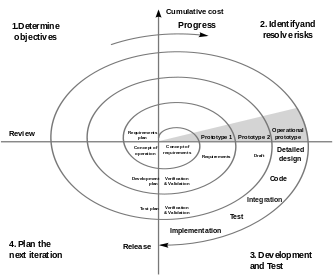
\includegraphics{spiralmodel.png}
  \caption{The Spiral model of development}
  \label{fig:spiral_model}
\end{figure}

To address the shortcomings of both methodologies, Boehm proposed the Spiral model which he noted as evolving based on the insights he had gained from applying the Waterfall model in large government projects.
It suggests a flexible approach based on the risk profile of each project which adopts suitable tools from one or more process based methodologies such as incremental development, the waterfall model, or evolutionary prototyping. A challenge with the Spiral model is that its core concepts have often been oversimplified leading to misconceptions and what Boehm terms `hazardous spiral look-alikes. This term refers to implemenations of the Spiral approach appear to have the all the required core components but in fact diverge and inviolate the one or more of the key principles of the model. To counteract this approach, Boehm stresses that projects using the spiral model should always display six invariants (items which are always required in every project) and he usefully provides examples where each invariant could be subject to an incorrect interpretation which would invalidate its meaning.

\begin{itemize}

\item \textbf{Define artifacts concurrently.} This invariant notes that concurrency is a better approach here as defining project artefacts sequentially increases the risk that the project does not meet stakeholder expectations.
\newpage
\item \textbf{Perform four basic activities in every cycle.}
At its core, the Spiral model emphasises four basic activities in each cycle of developmentm as follows:
\begin{itemize}
\item 1. Determine the objectives
\item 2. Identify and resolve risks 
\item 3. Development and test
\item 4. Plan the next iteration
\end{itemize}
\item \textbf {Risk determines level of effort.} It is the responsibility of the project team to determine how much effort should be spent on each project area, based on the perceived level of risk for the area. This decision should always be made based on a strategy of reducing the overall level of risk to the project.
\item \textbf {Risk determines degree of details} Based on a risk based approach, the team must make a determination as to how much detail needs to be gathered for each project artefact. For example, they should ensure they gather sufficient detail in relation to requirements areas where a detailed specification helps to reduce unpredictability and contribute to lowering the overall level of risk, for example in precisely defining the integration approach to be taken between hardware and software components. Conversely, project teams should feel entirely comfortable producing much less detail in relation to front requirements specifications in other areas which have a lower overall level of project risk, for example in relation to the design of the graphical user interface.
\item \textbf {Use anchor point milestones.} In the original specification of the spiral model, it did not initially include any project milestone assessments but from practical experience- again with a risk focussed approach- these were introduced to anchor project delivery to communicate progress updates to stakeholders.

\item \textbf {Focus on the system and its life cycle}
This invariant recommends that project managers and stakeholders take a long term view of the project life cycle and avoid an excessive focus in the initial stages of the project on the development of software code.
\end{itemize}
\newpage
\subsection {Agile}
The Agile manifesto emerged as a strong counterpoint to the various process driven approaches such as the Waterfall methodology and echoed many of the concerns and ideas of earlier iterative and incremental software development approaches.

The manifesto was written by 17 experienced software developers who convened in 2001 and drawing on their own experience of efficient software development principles, sought to define the guiding principles for the Agile Alliance. Central to their thinking was the notion that while they valued the items on the right hand column of the table above, they placed an even higher value on the items in the left hand column. For example, while they did see a value in developing documentation, they did not take this to the level of generating copious manuals for form's sake which would gather dust, not be kept up to date, and ultimately deliver little in terms of value to end users.

\begin{table}[]
\centering
\caption{The Agile Manifesto}
\label{my-label}
\begin{tabular}{|l|l|l|ll}
\cline{1-3}
Individuals and interactions & over & Processes and tools          \\ \cline{1-3}
Working software             & over & Comprehensive documentation \\ \cline{1-3}
Customer collaboration       & over & Contract negotiation        \\ \cline{1-3}
Responding to change         & over & Following a plan              \\ \cline{1-3}
\end{tabular}
\end{table}

The twelve principles of the Manifesto for Agile Software Development, which are reproduced verbatim below, have found wide acceptance among software developers, particularly in recent years as the time to market between releases in new areas of software development including mobile apps and online web applications needs to be much shorter than in traditional application development. Where traditional software houses could plan for new versions of their software to be released perhaps on an annual basis, which allowed sufficient time for testing, feedback and rework of code from testing to eliminate bugs, modern application development needs to focus on regularly adding new functionality. The `bite-sized' approach of Agile is a good fit for these rapid development requirements, allowing software development houses to iteratively plan and develop and test new releases of working software while allowing for frequent application updates to be responsive to customer needs, competitor actions or market conditions, often completing a development cycle within a short period of a few weeks.

These Agile principles have inspired many further iterative innovations in the field of software development giving rise to other approaches such as Extreme Programming, Lean Software Development (which has many parallels with Toyota's Lean Manufacturing System for vehicle manufacturer) and also resources and tools such as Kanban Boards, Scrum and DevOps tools. Some of the core project management methodologies such as PMBOK (The Project Management Book of Knowledge) and PMI (Project Management Institute )have also adapted to the emergence of Agile principles by defining specific Agile oriented project management methodologies. There are also mainstream training and certification options available for those who wish to pursue careers as Agile practioners or Scrum masters.



The \textbf{Manifesto for Agile Software Development} is based on twelve principles:
\begin{itemize}
\item Customer satisfaction by early and continuous delivery of valuable software
\item Welcome changing requirements, even in late development
\item Working software is delivered frequently (weeks rather than months)
\item Close, daily cooperation between business people and developers
\item Projects are built around motivated individuals, who should be trusted
\item Face-to-face conversation is the best form of communication (co-location)
\item Working software is the principal measure of progress
\item Sustainable development, able to maintain a constant pace
\item Continuous attention to technical excellence and good design
\item Simplicity—the art of maximizing the amount of work not done—is essential
\item Best architectures, requirements, and designs emerge from self-organizing teams
\item Regularly, the team reflects on how to become more effective, and adjusts accordingly
\end{itemize}
%----------------------------------------------------------------------------------------
%	Overview of fields reviewed and sources consulted
%       Review of SDLC, Agile vs Waterfall
%       UML Methodology- critical evaluation of UML
%       User Testing Approaches
%       MVC and alternative frameworks- why I chose MVC
% 	The Symfony Framework [and alternatives]
%----------------------------------------
\end{samepage}
\begin{samepage}
\newpage
\section {Initiation and Concept Development}

\subsection {Scope of Final Rostering and Scheduling Solution}
In order to address this deficiency, the IWA's Senior Management Team have mandated the IWA ICT team to work with internal stakeholders to define functional requirements and implement a competitive tender process to select and deploy a new software solution to enable IWA to manage rostering and the capture of time and attendance information in a more efficient manner.
The proposed solution will deliver the following functionality components to IWA:
\begin{itemize}
\item \textbf{A Rostering and Scheduling solution} for use by ALS Administrators, Coordinators and Support Officers. The proposed solution should also interface with the IWA Megapay payroll system. Finally, it should manage the customer billing process in relation to the care services provided to statutory and individual customers.
\item \textbf {A Mobile Application} to be used by PAs employed by IWA which should be capable of running on the iOS, Android and Windows Phone and thereby be suitable to run on the personal mobile devices of employees to avoid IWA having to supply company owned and funded devices on the corporate account. 
\item \textbf {Attendance Verification Mechanism via Mobile App}. A key requirement for the mobile application is that it provides a reliable and independent real-time verification of an employee’s attendance at a service visit location, together with timestamped confirmation of the length of time that was spent at the location.  This is required to satisfy IWA service level agreement obligations with its funders and to minimise the possibility of fraud.
\pagebreak
\item\textbf {Quotation/Proposals Generation.} The proposed enterprise solution should be capable of generating detailed and personalised Service proposals/ quotations where the coordinator can plan the service schedule for the service user, referencing each visit to the appropriate price card item to generate a completed quotation for the customer which shows the provisional service schedule and the projected weekly invoiced cost.
\item \textbf {Employee, Service User and Customer Portals.} IWA would also like to implement Service user and Employee portals which includes an authentication layer so that a service user or their family member can view upcoming service visits. Similarly, employees can view their upcoming roster visits to various service users including information such contact information, tasks to be completed etc. and a Customer portal where a funder can view invoices, schedules for upcoming service and validate completed visits by viewing validation timestamps of attendance.
\end{itemize}
\subsection {Scope of Prototype Solution}
As the prototype application is being fast tracked for user acceptance testing, this application has more limited scope and is primarily focussed on the backend Rostering and Scheduling solution and in particularly on examining in detail the user experience and optimal process and validation checks required by Coordinators and Administrators in handling various common service delivery scenarios.
The prototype will also attempt to model in a simplistic fashion the experience of portal layer users who will interact using various security limited roles such as employees, service users and customers although it will not attempt to fully implement the data privacy restrictions to be granted to each type of role- for example employees being unable to access the planned roster records for other employees to the fully robust extent that would be required in an enterprise level application.
The aspects of creation of a mobile app, integration of the mobile app with the backend rostering and scheduling and the verification of attendance via the mobile app are all considered as out of scope for the prototype application.
\end{samepage}
\pagebreak
\subsection {Feasibility Review}

\textbf{Risk Register for Project and Mitigation Actions}

\noindent\makebox[\linewidth]{\rule{\paperwidth}{0.4pt}}
\textbf{Risk: It may be challenging to find a solution which meets all of IWA’s requirements.}

Mitigation: In this regard, it will be necessary to prioritise those essential aspects of the new system’s functionality over ‘nice to have’ aspects

\noindent\makebox[\linewidth]{\rule{\paperwidth}{0.4pt}}
\textbf{Risk: Required project resources are not available or their input delays key project phases}

Mitigation: Agreement of IWA management to release key resources when required and provide backfill for the other work normally assigned to those resources

\noindent\makebox[\linewidth]{\rule{\paperwidth}{0.4pt}}
\textbf{Risk: The project takes longer to deliver or software/customisation costs are higher than anticipated.}

Mitigation: Detailed project planning and agreement of deliverables, costs and timelines with vendor. Prioritisation of scope and deliverables to ensure key functionality is delivered on time. 

\noindent\makebox[\linewidth]{\rule{\paperwidth}{0.4pt}}
\textbf{Risk: Solution does not fully meet IWA's requirements or becomes outdated as IWA's requirements change.}

Mitigation: Detailed agreement on deliverables/scope/cost for initial build and sign off of same with vendor. Comprehensive user acceptance testing and user sign off on agreed and tested functionality at key milestones. Design solution so that it is flexible to adapt to the key areas where IWA requirements may change e.g. payroll payment rate structure, billing rate structure, customer invoicing/reporting formats, additional functionality/ logic in the mobile app.

\noindent\makebox[\linewidth]{\rule{\paperwidth}{0.4pt}}
\textbf{Risk: Less than 100\% adoption by ALS teams, current manual processes persist at local level.}

Mitigation: Dedicated project manager for rollout phase working with local teams. Tight project planning and monitoring/direction from local ALS management teams to ensure project phases and adoption take place to plan. Structured training plan for staff using system and identification of staff who are struggling to adapt to the new process and provision of support by local ALS team leads to ensure they are brought up to speed.

\noindent\makebox[\linewidth]{\rule{\paperwidth}{0.4pt}}
\textbf{Risk: The prototype has limited value as it has marked differences in functionality or user interface from available production platforms which might be considered by IWA}

Mitigation: Focus on confirmation of required functionality over specific user interface features. Research commercial offerings and build some aspects of their user interface into prototype so that users get a realistic sense of what the finished product might look like
\newpage

\section {Requirements Analysis}
\subsection {Functional Requirements }

In this functional requirements section, we set out in simple terms what the prototype application will do. 

\begin{itemize}

\item \textbf {Managing Service Appointments.} For this application, the core objective of the system is to manage a series of appointments for care visits and to make sure that each one is covered, taking account of the relationships between service users and personal assistants.
\item \textbf {Documenting service user, customer, employee and office location and contact information.} The application should record (and show in the index and show views for each entity) the address and contact information for each employee, service user or office.
\item \textbf {Displaying service user roster as calendar plan.} The application should display the roster plan for each service user in a calendar plan (similar to an Outlook diary) format and allow the user to interact with and update each visit from that calendar view.
\item \textbf {Assigning service user, employee and customers to office locations.} The allow a user to indicate which IWA office is responsible for managing the relationship with a given service user, employee or customer.
\item \textbf {Geocoding addresses and Displaying Google Maps.} For each service user, employee and office. the system should integrate with Google Maps to obtain valid geocoordinates for the address and display this as a map on the view screen for each record.
\item \textbf{Assigning a Personal Assistant to a Service User.} A Personal Assistant (employee) will frequently be assigned as the `preference' (or regular) resouce to be sent to a given service user, based on a positive experience of working together. 
\item \textbf{Assigning a Personal Assistant as `Do Not Send' to a Service User.} Conversely, a negative experience from a previous visit may give rise to the need to designate that a given resource should not be sent to fulfil care visits for a particular service user. In this case, we would indicate this relationship by creating a `Do Not Send' association between the service user and the employee.
\item \textbf{Employee Unavailable TImes.} The system needs to document times when a  Personal Assistant (employee) is not available due to other commitments e.g. second job, family, college attendance and not show this employee as available when finding an employee to fill an unfilled slot 
\newpage
\item \textbf{Employee Absence.} The system needs to document times when a  Personal Assistant (employee) is on leave and unavailable to work and not show this employee as available when finding an employee to fill an unfilled slot 
\item \textbf{Employee Working.} The system needs to document times when a  Personal Assistant (employee) is assigned to a roster and therefore unavailable to work on other rosters. It should not show this employee as available when finding an employee to fill an unfilled 
\item \textbf{Roster required employees .} The system should store for each visit how many employees are required.
\item \textbf{Roster status.} When the number of assigned employees is less than the required quotient, the system should show a warning to this effect. When enough employees are assigned, the message should be updated to reflect this.
\item \textbf{Find an employee for an unassigned roster.} When the number of assigned employees is less than the required quotient, the system should allow a user to find a suitable employee to fulfil the visit, bearing in mind `do not send' relationships and filtering out employees who are working elsewhere, designated as unavailable at that time or recorded as being on an approved absence (holidays, sick leave etc.) at the time of the roster.
slot 
\end{itemize}
\subsection {Availability Requirements }

The system should be available over a web browser once the user has internet access. It should not rely on a client install of software on the user's machine nor should it require the user to use a VPN connection. 

\subsection {Security Requirements }
\begin{itemize}
\item \textbf{Encryption} The system should use an encrypted (https, SSL) connection to the server to ensure privacy of the data in transmission.
\item \textbf{Role Based Security} The system tag each uses to the IWA office that they are assigned to, and restrict that user to only be able to see service users, employees and customers associated with the office that the user is associated with (Note: out of scope for prototype deliverable)
\newpage
\item \textbf{Service User Portal User- Security} The system should allow user who are attached to the ServiceUser security role to login in and to only be able to see rosters for that service user (Note: out of scope for prototype deliverable)
\item \textbf{Employee Portal User- Security} The system should allow user who are attached to the Employee security role to login in and to only be able to see rosters to which that employee is assigned (Note: out of scope for prototype deliverable)
\item \textbf{Customer Portal User- Security} The system should allow user who are attached to the Customer security role to login in and to only be able to see rosters for which that customer is designated as the customer of the Roster visit (Note: out of scope for prototype deliverable)
\end{itemize}

\subsection {Use case specification}
The high-level use case specification aims to identify all the actors who will use a system and what actions they can take in that system.

\subsection {Detailed Use Case Analysis}
 \begin{figure}[h!]
  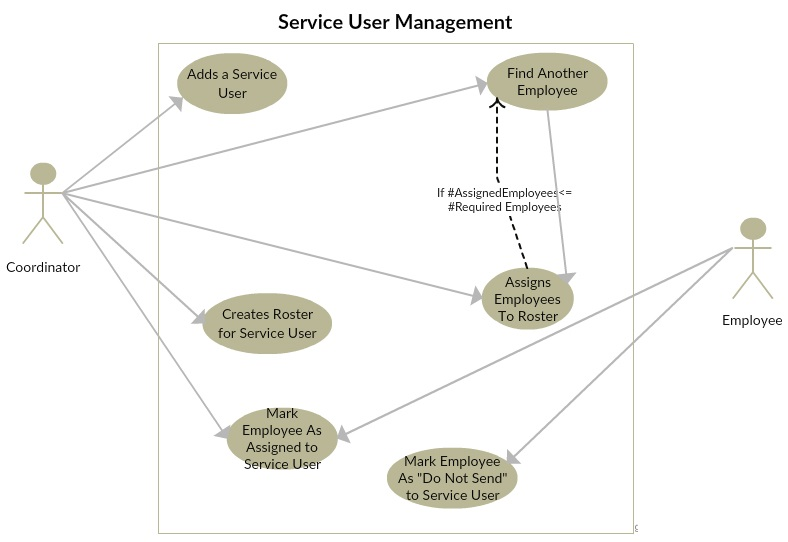
\includegraphics[scale=0.8]{rosterusecase.jpg}
  \caption{Roster Use Case}
  \label{fig:roster use case}
\end{figure}
The following detailed use cases have been identified for the prototype application. As many of the use cases relate to standard CRUD (Create, Read, Update, Delete) functionality for each entity for which it is envisaged that using the Symfony templating approach to initially scaffold the generic controller and related views and form type classes,a generic use case for each of these four standard functions has been created to avoid duplication and repetition. As noted, this generic use case- for example new() entity record- is therefore applicable to all of the individual entities noted, and any particular variations (for example passing parameters to identify a related entity context) are noted in the use case where appropriate
\begin{usecase}
    \addheading{Title}{User login}
  \addheading{Description}{User supplies credentials to login}
  
  \addheading{Actor}{User} 
  \addrow{Precondition}{User must not be logged in ie is currently authenticated as anonymous user}
  \addrow{Postcondition}{User is authenticated having supplied correct password and holds one or more security role}
  \addmulrow{Basic Flows (M)}{\item User navigates to login area via base template button which is visible on all pages\ldots
                                  \item User enters username and password and clicks login\ldots
                                  \item Controller method checks username and password against user repository. If credentials are matched to repository logs user in and set the user as authenticate, allocating any roles held by that user
                                  \item If credentials are not matched to repositoryare display login failed message and redisplay the login screen\\ldots}
  \addmulrow{Alternate Exception Flows (M)}{\item User who is not logged in attempts to access a secured resource and is automatically rerouted to the login screen\ldots}
                                  
\end{usecase}

\begin{usecase}
    \addheading{Title}{User registration}
  \addheading{Description}{User a username and password and creates a new user account}
  
  \addheading{Actor}{User} 
  \addrow{Precondition}{User must not be logged in ie is currently authenticated as anonymous user}
  \addrow{Postcondition}{User is authenticated having supplied correct password and holds one or more security role. User credentials are updated in the database for future visits}
  \addmulrow{Basic Flows (M)}{\item User navigates to register area via base template button which is shown on all pages when the user is not currently logged in \ldots
                                  \item User enters username and password and clicks login\ldots
                                  \item Controller method checks username and password against user repository. If credentials supplied are valid, and do not duplicate an existing user account the user is set to a logged in stage and the database is updated
                                  \item If credentials are matched to an existing user record in the repository display the registration failed message and redisplay the registration form screen\\ldots}
  \addmulrow{Alternate Exception Flows (M)}{\item None\ldots}
                                  
\end{usecase}

\begin{usecase}

    \addheading{Title}{User accesses index view of entity records }
  \addheading{Description}{User can view index list of one of type Customer, Employee, Roster Assignment, Service User, Service User Assignment, Employee Absence Times, Employee Unavailability, Do Not Send, Office records. This is a reusable use case mapped to multiple Entities,all created using the Symfony templating approach}
  \addheading{Actor}{User} 
  \addrow{Precondition}{User must be logged in and hold an appropriately authorised security role}
  \addrow{Postcondition}{N/A.}
  \addmulrow{Basic Flows (M)}{\item User navigates to index view and can see all customer records\ldots
                                  \item User clicks on Edit link and can view a single page view screen of the selected record\ldots}
  \addmulrow{Alternate Exception Flows (M)}{\item User is not logged in. On routing to area, system routes User to user login screen and denies permission to resource until they have successfully authenticated using an account holding the appropriate  role\ldots
                                   \item User attempts to route to a record that doesn't exist and is shown error 404 not found\ldots
                                   \item Attempt to retrieve entity records failed at database level. redisplay previous screen and advise user that an error was encountered and suggest that they retry the effort\ldots
                                   \item User authenticates but does not hold an appropriate role to access the index view. Display 403 forbidden exception message\ldots}

\end{usecase}

\begin{usecase}
    \addheading{Title}{User views individual entity item}

  \addheading{Description}{User can select view an individual item of type Customer, Employee, Roster Assignment, Service User, Service User Assignment, Employee Absence Times, Employee Unavailability, Do Not Send, Office records}
  \addheading{Actor}{User} 
  \addrow{Precondition}{User must be logged in and hold an appropriately authorised security role}
  \addrow{Postcondition}{N/A.}
  \addmulrow{Basic Flows (M)}{\item User navigates to that record and can see all attributes of that entity record on a single page\ldots}
  \addmulrow{Alternate Exception Flows (M)}{\item User is not logged in. On routing to area, system routes User to user login screen and denies permission to resource until they have successfully authenticated using an account holding the appropriate role\ldots
                                   \item User attempts to route to a record that doesn't exist and is shown error 404 not found\ldots
                                   \item Attempt to retrieve selected record failed at database level. redisplay index and advise user that an error was encountered and suggest that they retry the effort\ldots
                                    \item User authenticates but does not hold an appropriate role to view the entity item. Display 403 forbidden exception message\ldots}

\end{usecase}

\begin{usecase}
    \addheading{Title}{User can create a new entity record }
  \addheading{Description}{User can create a new record of type Customer(s), Employee, Roster Assignment, Service User, Service User Assignment, Employee Absence Times, Employee Unavailability, Do Not Send, Office records. This is a reusable use case mapped to multiple Entities,all created using the Symfony templating approach}
  \addheading{Actor}{User} 
  \addrow{Precondition}{User must be logged in and hold an appropriately authorised security role}
  \addrow{Postcondition}{The newly created record is now saved to the database}
  \addmulrow{Basic Flows (M)}{\item User navigates to index view and clicks the new button or navigates from a related entity (see Alternate Flow below)\ldots
                                  \item User clicks on New link and can view a single page form screen with empty attribute controls for the selected record type\ldots}
  \addmulrow{Alternate  Flows (M)}{\item from service user record, user clicks on a button for new roster or assign employee or mark as do not send. Or from employee, user clicks on add unavailability time or employee absence period. User is routed to special version of the New() action for that entity which accepts either an employee or service user object as a parameter and method binds new entity record to have service user or employee context as an associated foreign key when saving newly created record)\ldots}
  \addmulrow{Alternate Exception Flows (M)}{\item User is not logged in. On routing to area, system routes User to user login screen and denies permission to resource until they have successfully authenticated using an account holding the appropriate role\ldots
                                                                      \item User authenticates but does not hold an appropriate role to access the index view. Display 403 forbidden exception message\ldots
                                                                      \item Attempt to save new record failed at database level. redisplay new record form with previously entered form data and advise user that an error was encountered and suggest that they retry the effort\ldots}

\end{usecase}

\begin{usecase}
    \addheading{Title}{User can edit an entity record }
  \addheading{Description}{User can retrieve and edit an existing record of type Customer(s), Employee, Roster Assignment, Service User, Service User Assignment, Employee Absence Times, Employee Unavailability, Do Not Send, Office records. This is a reusable use case mapped to multiple Entities,all created using the Symfony templating approach}
  \addheading{Actor}{User} 
  \addrow{Precondition}{User must be logged in and hold an appropriately authorised security role}
  \addrow{Postcondition}{The updated record is now saved with changes made to that single entity record updated to the database}
  \addmulrow{Basic Flows (M)}{\item User navigates to index view and clicks the edit button \ldots
                                  \item User is routed to a single page form screen with attribute controls for the selected record type prepopulated with the previously saved values retrieved from the database\ldots
                                  \item User makes changes to the field values and clicks update or save. The changes are validated and then saved to the database\ldots}
  \addmulrow{Alternate  Flows (M)}{\item The user cancels the attempt to edit the record and turns to the (non editable) form version of the entity\ldots}
  \addmulrow{Alternate Exception Flows (M)}{\item User is not logged in. On routing to area, system routes User to user login screen and denies permission to resource until they have successfully authenticated using an account holding the appropriate role\ldots
                                                                      \item User authenticates but does not hold an appropriate role to access the index view. Display 403 forbidden exception message\ldots
                                                                      \item Attempt to save new record failed at database level. redisplay new record form with previously entered form data and advise user that an error was encountered and suggest that they retry the effort\ldots}

\end{usecase}

\begin{usecase}
    \addheading{Title}{User can delete a new entity record }
  \addheading{Description}{User can delete a single entity record of type Customer(s), Employee, Roster Assignment, Service User, Service User Assignment, Employee Absence Times, Employee Unavailability, Do Not Send, Office records. This is a reusable use case mapped to multiple Entities,all created using the Symfony templating approach}
  \addheading{Actor}{User} 
  \addrow{Precondition}{User must be logged in and hold an appropriately authorised security role}
  \addrow{Postcondition}{The deleted record is removed from the database.}
  \addmulrow{Basic Flows (M)}{\item User navigates to index view and clicks the delete button \ldots
  \item the selected record is removed from the database\ldots}
  \addmulrow{Alternate  Flows (M)}{\item The user clicks the delete button when in the view/show mode and having previously selected an individual record to view/show\ldots}
  \addmulrow{Alternate Exception Flows (M)}{\item User is not logged in. On routing to area, system routes User to user login screen and denies permission to resource until they have successfully authenticated using an account holding the appropriate role\ldots
                                                                      \item User authenticates but does not hold an appropriate role to access the index view. Display 403 forbidden exception message\ldots
                                                                      \item Attempt to save new record failed at database level. Redisplay current record and advise user that an error was encountered and suggest that they retry the effort\ldots}

\end{usecase}


\begin{usecase}
    \addheading{Title}{Check for a Do Not Send relationship between an employee and a service user}
  \addheading{Description}{When saving an assignment of an employee to a roster, check first that a do not send relationship has not already been defined for that employee.}
  \addheading{Actor}{User} 
  \addrow{Precondition}{User must be logged in and hold an appropriately authorised security role. This method is called when assigning an employee to a roster record}
  \addrow{Postcondition}{The roster assignment record is updated with the relevant employee entity from the database.}
  \addmulrow{Basic Flows (M)}{\item User assigns an employee to a record. \ldots
  \item If no do not send relationship exists between the service user and the employee, save the selected roster assignment record to the database\ldots}
  \addmulrow{Alternate  Flows (M)}{\item If a do not send relationship does exists between, do not save the roster assignment and advise the user that the change has not been saved because of the do not send relationship\ldots}
  \addmulrow{Alternate Exception Flows (M)}{\item User is not logged in. On routing to area, system routes User to user login screen and denies permission to resource until they have successfully authenticated using an account holding the appropriate role\ldots
                                                                      \item User authenticates but does not hold an appropriate role to access the index view. Display 403 forbidden exception message\ldots
                                                                      \item Attempt to save new record failed at database level. Redisplay current record and advise user that an error was encountered and suggest that they retry the effort\ldots}

\end{usecase}

\begin{usecase}
    \addheading{Title}{Display available employees for a roster}
  \addheading{Description}{When a roster does not have enough employees assigned, show available employees to the user and allow them to select one.}
  \addheading{Actor}{User} 
  \addrow{Precondition}{User must be logged in and hold an appropriately authorised security role. The roster must not have sufficient employee resources attached}
  \addrow{Postcondition}{None.}
  \addmulrow{Basic Flows (M)}{\item User clicks on the Find An Employee To Assign button on a roster record \ldots
  \newpage
  \item The controller method retrieves all employees and then filters out employee who have a do not send relationship to that service user\ldots
  \item From the residual array of employee objects, the controller method filters out employee who are not available at that time due to being assigned elsewhere\ldots
    \item From the residual array of employee objects, the controller method filters out employee who have recorded that they are unavailable at that time\ldots
        \item From the residual array of employee objects, the controller method filters out employee who have an absence recorded which overlaps with the roster time\ldots
            \item Finally, the residual array of available employee objects are displayed to the user and the user can select an individual employee record from the displayed list and click the assign button\ldots}
  \addmulrow{Alternate  Flows (M)}{\item There are no available employees and the user navigates away from the page\ldots}
  \addmulrow{Alternate Exception Flows (M)}{\item User is not logged in. On routing to area, system routes User to user login screen and denies permission to resource until they have successfully authenticated using an account holding the appropriate role\ldots
                                                                      \item User authenticates but does not hold an appropriate role to access the  view. Display 403 forbidden exception message\ldots
                                                                      \item Attempt to assign the selected employee to the roster record failed at database level. Redisplay current record and advise user that an error was encountered and suggest that they retry the effort\ldots}
\end{usecase}

\begin{usecase}
    \addheading{Title}{Get Mapping coordinates for address}
  \addheading{Description}{Use call to Google Maps API to retrieve geocoordinates for an address. Reusable factory method which accepts either an employee, service user or office object and geocodes the address for that object}
  \addheading{Actor}{User} 
  \addrow{Precondition}{User must be logged in and hold an appropriately authorised security role. The object to be geocoded must have an address}
  \addrow{Postcondition}{The latitude and longtitude of the object's address are saved to the database.}
  \addmulrow{Basic Flows (M)}{\item User clicks on the Geocode button from the show screen of an employee, service user or office entity record\ldots
  \newpage
  \item The controller method sends an appropriate API call to the Google Maps location service which returns a valid set of the coordinates for the address\ldots}
  \addmulrow{Alternate  Flows (M)}{\item If Google Maps cannot locate the coordinates return and save an empty of coordinate values as latitude and longtitude\ldots}
  \addmulrow{Alternate Exception Flows (M)}{\item User is not logged in. On routing to area, system routes User to user login screen and denies permission to resource until they have successfully authenticated using an account holding the appropriate role\ldots
                                                                      \item User authenticates but does not hold an appropriate role to access the geocoding  view. Display 403 forbidden exception message\ldots
                                                                      \item Attempt to assign the newly obtained coordinates failed at database level. Redisplay current record and advise user that an error was encountered and suggest that they retry the effort\ldots}
\end{usecase}

\begin{usecase}
    \addheading{Title}{Assign user role(s) }
  \addheading{Description}{Assign role(s) to a user}
  \addheading{Actor}{Administrator} 
  \addrow{Precondition}{User must be logged in and hold an appropriately authorised security role.}
  \addrow{Postcondition}{User role is updated against the appropriate user record.}
  \addmulrow{Basic Flows (M)}{\item Administrator clicks on Assign User Role button from the Admin button shown only to Administrator role\ldots
  \newpage
  \item Administrator selects the requried role and clicks update\ldots}
  \addmulrow{Alternate Exception Flows (M)}{\item User is not logged in. On routing to area, system routes User to user login screen and denies permission to resource until they have successfully authenticated using an account holding the appropriate role\ldots
                                                                      \item User authenticates but does not hold an appropriate role to access the Administrator  view. Display 403 forbidden exception message\ldots
                                                                      \item Attempt to assign the newly obtained coordinates failed at database level. Redisplay current record and advise user that an error was encountered and suggest that they retry the effort\ldots}
\end{usecase}

\begin{usecase}
   \addheading{Title}{Password reset}
  \addheading{Description}{Reset the password of a user}
  \addheading{Actor}{Administrator} 
  \addrow{Precondition}{User must be logged in and hold an appropriately authorised security role.}
  \addrow{Postcondition}{New password value is updated against the appropriate user record.}
  \addmulrow{Basic Flows (M)}{\item Administrator clicks on Reset Password button from the Admin button shown only to Administrator role\ldots
  \newpage
  \item Administrator selects the user whose password needs to be reset and then enters in a new password\ldots
  \item New password is saved to the database\ldots}
  \addmulrow{Alternate Exception Flows (M)}{\item User is not logged in. On routing to area, system routes User to user login screen and denies permission to resource until they have successfully authenticated using an account holding the appropriate role\ldots
                                                                      \item User authenticates but does not hold an appropriate role to access the Administrator  view. Display 403 forbidden exception message\ldots
                                                                      \item Attempt to save the new password failed at database level. Redisplay current record and advise user that an error was encountered and suggest that they retry the effort\ldots}
\end{usecase}

\end{samepage}
\newpage
\section{Design Specification}
\subsection {System Design Document}
\subsubsection{Hardware Architecture- Prototype Application}

Considerations for the Prototype Application: It is envisaged that the prototype system will be hosted initially on the author's own personal web hosting for prototyping purposes and with a limited intiial user base. This will incorporate a web front end, with a successful user login required to access most parts of the application. The system will utiilise a MySQL backend database and the web application will interact with this database layer through Symfony/Doctrine repository classes (see below for more information)
\subsubsection{Hardware Architecture- Production Appplication}

Considerations for the Production Application: It is envisaged that the production system will incorporate a load balanced web application server with a backend database though a private cloud hosted system is considered to be ideal for the usage scenario. Further consideration of the hardware/ infrastructure environment will depend on the specific solution chosen as a result of the procurement process and is deferred here until this has been completed.

\subsection {Software Development Document}
\subsubsection{Design considerations}
Given the requirement to rapidly complete and deliver a prototype application for user acceptance testing, the ability to deliver a basic working application in a short timeframe becomes a paramount consideration. A second consideration is to ensure an appropriate separation of concerns between the front end application (the view that is presented to the user through the user interface), controller methods where the application business logic is applied (for example determining which employees are actually available to cover an unfilled roster) and lower level data level operations such as retrieving, adding or updating a record from/to the back end database.
\subsubsection{Model View Controller}

The \textbf{Model View Controller} approach as shown in Figure 3 below is a widely used application development approach which meets the above requirements and also helps to enforce a degree of rigour and structured design to the code base for the application.

 \begin{figure}[h!]

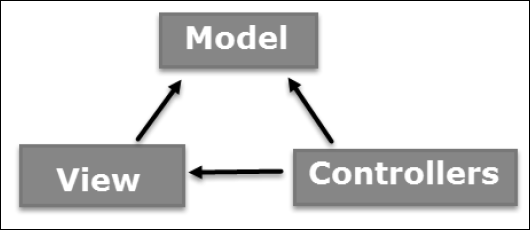
\includegraphics{mvc.jpg}
  \caption{The Model View Controller}
  \label{fig:model view controller}
\end{figure}
In this approach there are three main components in the architectural pattern each of which serves a different purpose but works in conjunction with the other two components, while achieving the requirement for separation of concerns.

\begin{itemize}
\item \textbf{Model} represents an object with each entity's attendant data attributes 
\item \textbf{View} represents the presentation layer to the user of the data which is stored in the model
\item \textbf{Controller} represents the connecting layer between the model and the view. It allows the data flow into the model object and keeps the presentation of the data in the viewup to date when the actual data in the object changes. It can act on both the model and the view and keeps the view and the model separate from one another.
\end{itemize}

\subsubsection{Comparison of a Web Development Framework}
The following different web development frameworks- each of which are suitable to produce dynamic, data driven web pages- were evaluated in the search to find a suitable platform on which to build the prototype application. All three platforms examined offer the ability for server side logic within an application.
\begin{itemize}
\item \textbf{ASP.NET MVC} is the Microsoft led development stack based on the .Net framework which is a widely used set of web development tools . It offers a strong integrated development environment (IDE) in Visual Studio which is freely available in the Community edition for non commercial use cases. It uses a combination of HTML, Razor, a proprietary Microsoft syntax used for developing views and C\# for controller and repository and other non view related classes. It supports an MVC led approach with  scaffolding of views and controllers based on having first creating a model with the relevant entity classes. It also integrates well with Azure web services, Microsoft's cloud stack where Visual Studio allows you to easily deploy web applications from a development environment. Asp.Net also includes the Entity Framework which essentially allows a code free, scaffolded approach to working with the database, driven entirely from the data model in your application. It also supports a test driven approach and integrates with a wide variety of third party components through a vibrant Nuget package marketplace.
\item \textbf{Symfony} is a widely used web development framework developed by Fabien Potencier and distributed as open source tools which also supports the MVC approach to separatino of concerns. It uses the very flexible Twig templating engine (which in the author's opinion is easier to use than Razor!) and allows users to adopt a flexible approach to selecting which Symfony components they choose to use in a given application. As Symfony has reached a wide degree of developer adoption, achieving 500 million downloads of the framework in 2016, it is widely supported with a significant choice of different add-on components (termed bundles in the Symfony domain) which are available to its developer community. Symfony uses PHP as its main code language and allows developers to easily scaffold views and controllers based on the creation of an entity model. It also supports a scaffolded approach to interacting with databases, similar in approach to Entity Framework through the use of command line tools which validate and update your database as required. Because Symfony uses the Doctrine ORM (Object Relational Mapping)which abstacts database layer operations from the rest of the application it supports MySQL and various other database platforms including SQLite, PostgreSQL and Microsoft SQL server.

An interesting twist on the Symfony approach, which is essentially a full stack framework, is the Silex approach, which uses elements of the Symfony framework (and a related library called Pimple) without requiring the developer to fully utilise all of the Symfony components and instead beginning with a skeleton framework which is much smaller and lighter in size than the full Symfony framework. When using Silex, a developer still has the flexibility to add in other components from the larger Symfony stack as the requirements of their application grow. One aspect about Symfony to note here is that the author notes some commentary from the developer community online which would suggest that Symfony is an ideal approach for small to medium web applications but its highly component driven approach can result in some performance impacts when used in very large scale deployments. Symfony also supports a test driven approach, both through using the test classes built into the application framework but also through its tight integration with the PHPUnit testing framework.
\item \textbf{Node.js} is a third very commonly used web development open source framework developed by Ryan Dahl which runs on a Javascript run time environment which allows for Javascript code to be executed server side. Again, Node.js also supports the MVC approach to separation of concerns. This innovations provided by Node.js allow Javascript, traditionally a client side scripting language, to be run server side and has become one of the core components driving the "Javascript everywhere'' development paradigm. Node.js supports a similar ORM driven approach to database operations resulting in a wide variety of relational and non relational databases being supported. Similar to ASP.Net and Symfony, Node.js has a number of different templating languages including Jade, blade, Mustache and Handlebars JS. It has also achieved wide acceptance among developers and has an extensive library available of reusable components, which serve to significantly reduce the requirement for developers to write their own code for commonly used operations. Node.js is perceived as an advanced level language with a significant learning curve to be overcome for developers migrating to the platform. An advantage of Node.js is that it does not create a lock on server resources and scales very well to large scale applications, working particularly well in scenarios which require real time processing. Corporate users of Node.js include LinkedIn, Microsoft, Netflix and Paypal.
\end{itemize}
\subsubsection{Choice of a Web Development Framework}

Though it was very instructuve to learn more about Node.js as part of the research for the project, the perceived difficulty level associated with this platform and the author's lack of previous exposure to it meant that it was not an ideal choice for a student project, particularly as there was a requirement for a rapid delivery of a prototype application for user testing. The author had some previous exposure to ASP.NET MVC and viewed this as viable choice for the application. However, using PHP/Symfony was a better fit given that the syllabus for the HDip in Computing that had been undertaken over the past 2 years had included significant exposure to PHP and the project/prototyping requirement afforded the author an opportunity to gain a familiarity with Symfony. It was also very helpful that the author's supervisor on this project had produced some excellent learning materials on the Symfony platform which greatly assisted in getting to grips with the new platform. A minor criticism of the Symfony platform is that while the documentation is generally excellent and extremely comprehensive, it can be somewhat challenging for developers migrating to the platform for the first time to get over the initial learning curve and get up and runniing in developing their very first Symfony application.

In fact, the first draft of the prototype application for this project was initially built on the Silex platform and as some of the requirements for implementation of a robust security model and the advantages of the scaffolding approach offered by Symfony came to light, it was determined to be useful to rebuild the entire prototype application on the full Symfony stack. It was most instructive to the author to note that having built the application on the Silex plaform originally, the second build on the Symfony platform, which was completed from scratch without reuse of any of the Silex application, took approximately 30\% of the time originally taken to build the Silex application, due in no small part to the automated scaffolding approach which Symfony offers to automate the construction of CRUD controller functions as well templated views. 
\subsubsection{Examples of some code efficiencies available in Symfony}
The author was very impressed with the following Symfony capabilities which among others were noted to substantially save time in manual coding tasks:
\textbf{Twig Templating }allows calling server side code in a format which is less verbose and easier to manage than embedding PHP code among the HTML code in your presentation view. A simple example is included here. Note also the concise way that the Annotation of related classes referred to below allows you to access attributes of a related class, in this case the mobile telephone property of the related employee class.

\begin{verbatim}


  <td>{{ assignedEmployee.employeeId }}</td>
  <td>{{ assignedEmployee.employeeId.mobileTelephone }}</td>

\end{verbatim}
The \textbf{Annotation capabilities} allow foreign keys to be defined in annotations to a given class or attribute which are automatically created in the underlying database, as follows:

 \begin{verbatim}

/**
 * Roster
 *
 * @ORM\Table(name="roster")
 * @ORM\Entity(repositoryClass=
 "AppBundle\Repository\RosterRepository")
 */
class Roster

{
    /**
     * @ORM\Column(type="integer")
     * @ORM\Id
     * @ORM\GeneratedValue(strategy="AUTO")
     */
    private $id;

    /**
     * @ORM\ManyToOne(targetEntity=
     "AppBundle\Entity\ServiceUser")
     * @ORM\JoinColumn(name="serviceUserId", 
     referencedColumnName="id")
     */
    private $serviceUserId;
\end{verbatim}
 
The \textbf{Form Type/ Builder} classes allow an entity's data entry/update form to be automatically scaffolded based on the entities data attributes as defined in its model. For example rather than having to create each an individual label and attribute for each property of the customer class, Symfony automatically scaffolds this using very simple syntax as follows:
 
 \begin{verbatim}
     public function buildForm(FormBuilderInterface $builder, 
     array $options)
    {
        $builder->add('customerName')->add('addressLine1')->
        add('addressLine2')->add('addressLine3')->
        add('eirCode')->add('landlineTelephone')->
        add('mobileTelephone')->add('isActive')->
        add('mainContact')->
        add('countyPostcode')->add('managingOffice');
    }

    /**
     * {@inheritdoc}
     */
    public function configureOptions(OptionsResolver $resolver)
    {
        $resolver->setDefaults(array(
            'data_class' => 'AppBundle\Entity\Customer'
        ));
    }
    
\end{verbatim}

Then in the actual presentation view, the syntax required to build the form, in this case an Edit form for a customer record, is extremely concise and the scaffolding approach automatically updates the form as the model of the entity class changes, An Example of calling the formbuilder from a view is shown in the Twig template as follows:

\begin{verbatim}
{ form_start(edit_form) }}
    {{ form_widget(edit_form) }}
    <input type="submit" value="Edit"/>
    {{ form_end(edit_form) }}
\end{verbatim}
Where it's necessary to extend the logic of an individual entity's form type, Symfony provides an extensive libary of FormTypes which can be used and overridden as required. For example, the EntityType class allows you to wire the contents of a dropdown control to the list of objects in another entity- or in this case,the ChoiceType allows you to define in your FormType class the contents of a drop down control together with both the values and labels for the dropdown control. An example of how you can extend the logic of the formtype is this instance where the form needed to include or not include a roster date field depending whether the submitted form data included a value in the posted \_REQUEST attribute which represented the posted form data. In this scenario, the form builder needed to handle both a new record being created which routes to the generic form without a roster date prepopulated, and a new record being created from a calendar with the specific date in question already set by the user clicking +new in the on a specific date.
This can be handled using logic in the formbuilder as follows:
\begin{verbatim}

    public function buildForm(FormBuilderInterface $builder,
     array $options)
    {
        $timezone = new \DateTimeZone("Europe/Dublin");

        if (isset ($_REQUEST['rosterDate'])) {
        $builder->add('serviceUserId', EntityType::class, 
        array('class' => 'AppBundle:ServiceUser',
            'data' => $options['serviceUser']))
            ->add('rosterStartTime', DateTimeType::class,
                array('date_widget' => "single_text",
                    'time_widget' => "single_text",
                    'data' => new \DateTime($_REQUEST['rosterDate'], 
                    $timezone)))
            ->add('rosterEndTime', DateTimeType::class, 
            array('date_widget' => "single_text",
                'time_widget' => "single_text",
                'data' => new \DateTime($_REQUEST['rosterDate'],
                 $timezone)))
            ->add('numberResourcesNeeded',
             ChoiceType::class, array(
                'choices' => array(
                    '0' => '0',
                    '1' => '1',
                    '2' => '2',
                    '3' => '3'),
                'required' => true,
                'placeholder' => 'Choose How Many
                 Resources Are Needed',
                'empty_data' => null
            ))
            ->add('customerId');
    } else {
            $builder->add('serviceUserId', EntityType::class, 
            array('class' => 'AppBundle:ServiceUser',
                'data' => $options['serviceUser']))
                ->add('rosterStartTime', DateTimeType::class,
                    array('date_widget' => "single_text",
                        'time_widget' => "single_text",
                    ))
                ->add('rosterEndTime', DateTimeType::class,
                 array('date_widget' => "single_text",
                    'time_widget' => "single_text",
                ))
                ->add('numberResourcesNeeded', 
                ChoiceType::class, array(
                    'choices' => array(
                        '0' => '0',
                        '1' => '1',
                        '2' => '2',
                        '3' => '3'),
                    'required' => true,
                    'placeholder' => 'Choose How Many Resources Are Needed',
                    'empty_data' => null
                ))
                ->add('customerId');
        }
    }
\end{verbatim}
 
The \textbf{Dynamic Query} capabilities of Symfony the Doctrine ORM can obviate the need to create specific views at a database level of entity classes where a (presentation level) view needed to present de-normalised data to the user. As an example of this capability, on the assumption that a \textbf{rosterassigned} entity exists and this has a foreign key attribute which relates to a roster entity. In this case there's a many to one entity relationship as one or more employees may be assigned via a rosterassignment record to a single roster entity. Once this relationship exists, it's possible to dynamically query the entity to retrieve only assignments which have a relationship to a specific roster, as follows:

\begin{verbatim}$assignedEmployees = $em->
getRepository('AppBundle:RosterAssignedEmployee')
->findByRosterId($roster->getId());
\end{verbatim}
\
The \textbf{Query builder} feature offers a powerful and flexible range of default Doctrine ORM queries similar to the findByRosterId() one noted above. These cater for most scenarios but it is also possible to create your own queries which resemble an SQL type logic (there's also a Doctrine Query Language which resembles the T-SQL query approach to database queries even more closely, but the author did not find a need for this in this project) which allows you to create your own custom queries when the need arises. 

For example, this query accepts a datetime object and a service user object as input parameters and checks to see if there are any rosters for the service user starting at any time in the 24 hour period of the datetime object provided. This query is used in a section of the Show view for a service user which displays a calendar control in a table control showing each as a line of table data. It then returns a true or false value to the calling method depending on whether or not a roster was found for that day.
The logic of the custom getByDate() query is as follows:
\begin{verbatim}
     
// this doctrine filter is used by the for loop in the show
// method of the service user controller.
//for each checked date in the for loop it checks to see if 
//that service user has any rosters starting in that 24 hour period.
    public function getByDate(\DateTime $date, ServiceUser $serviceUser)
    {
        $from = new \DateTime($date->format("Y-m-d") . " 00:00:00");
        $to = new \DateTime($date->format("Y-m-d") . " 23:59:59");
       
        $qb = $this->createQueryBuilder("roster");
        $qb->andWhere($qb->expr()
        ->between('roster.rosterStartTime', ':date_from', ':date_to'))
         ->andWhere("roster.serviceUserId= " . $serviceUser->getId());
        $qb->setParameter('date_from', $from,
         \Doctrine\DBAL\Types\Type::DATETIME);
        $qb->setParameter('date_to', $to, 
        \Doctrine\DBAL\Types\Type::DATETIME);
        $result = $qb->getQuery()->getResult();
        return $result;
    }
}  
\end{verbatim}

\subsection { Entity Relationship Diagram}
Based on the review of the use cases together with workshops with the subject matter experts provided within the Assisted Living Services team a map of the required classes for the application together with the properties and methods required for each class was created. This was then modelled into an initial Entity Relationship Diagram which is included on the next page.
 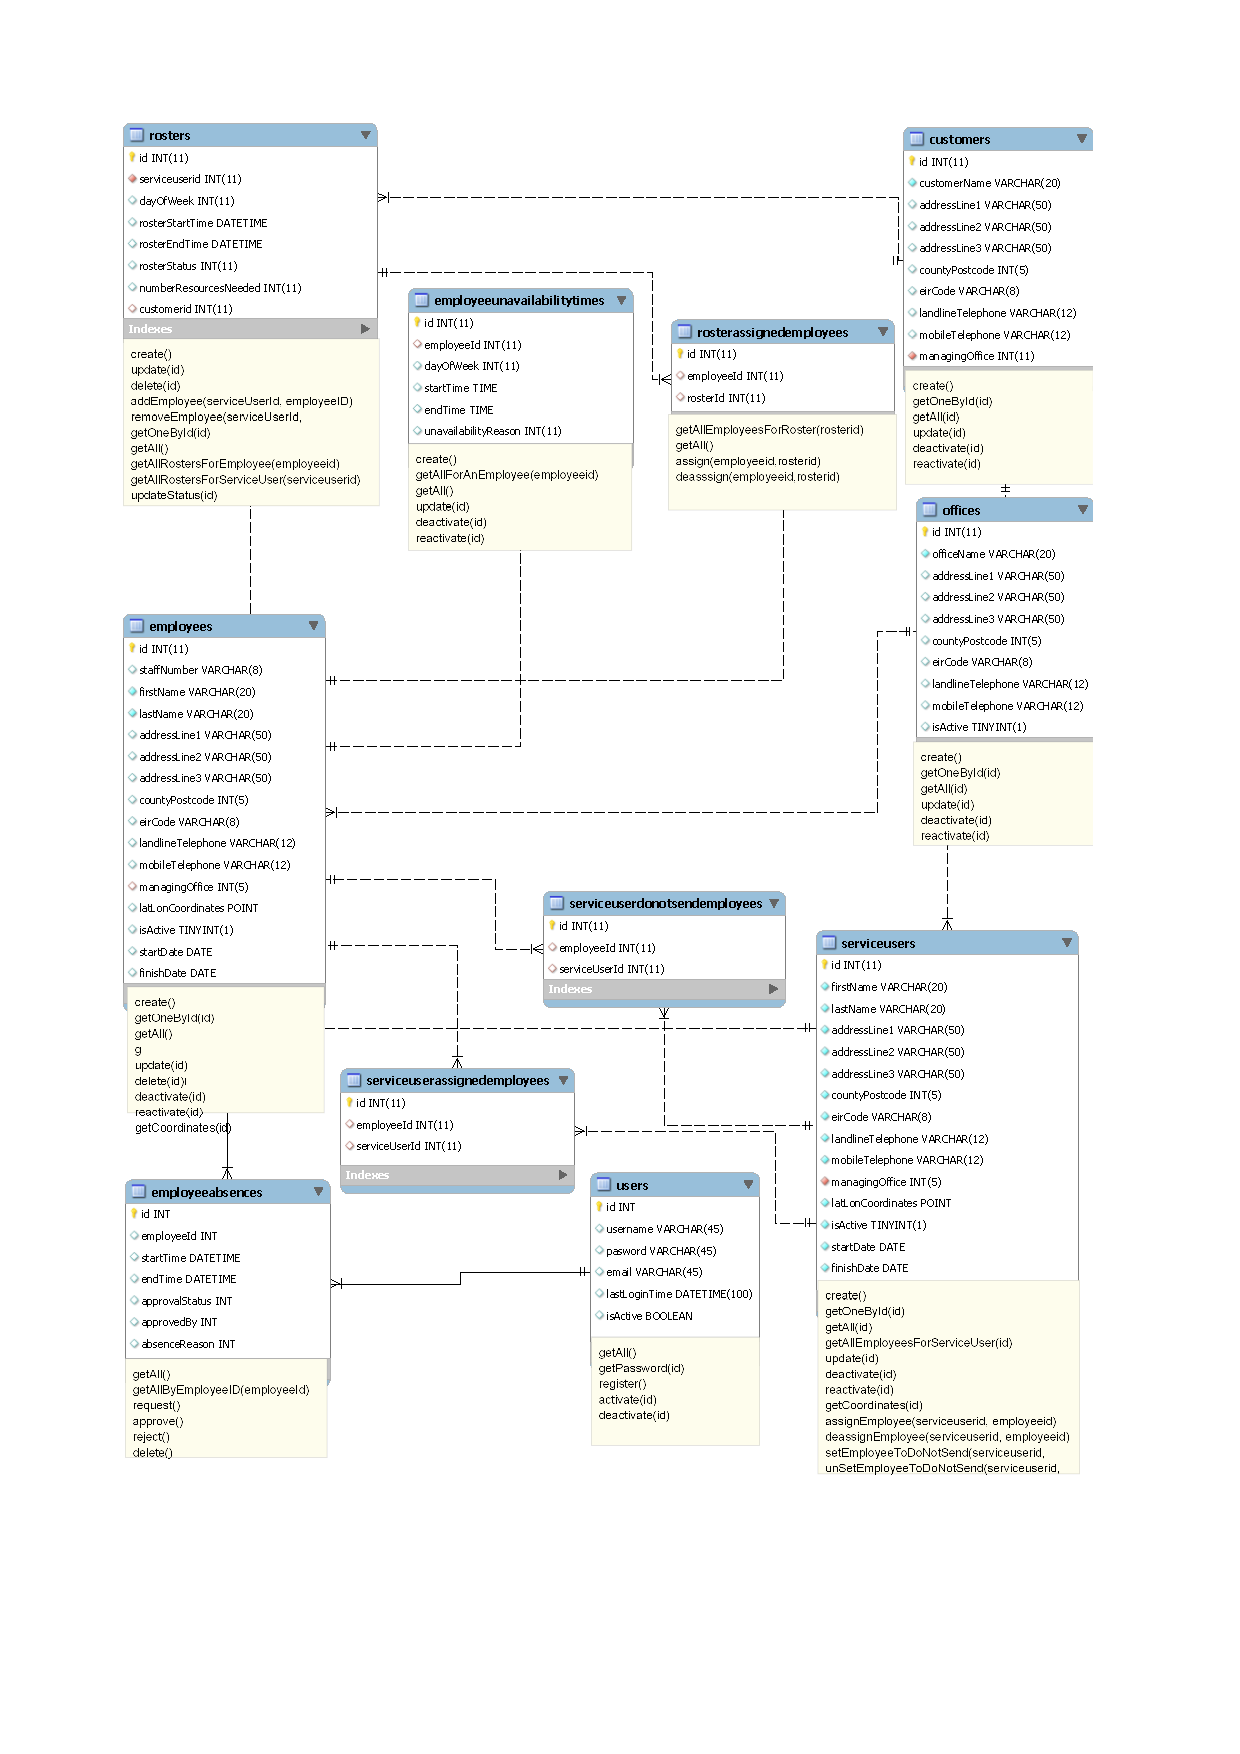
\includepdf[]{erd.pdf}

\subsection { Code Organisation for Project}
As the prototype application, though less full featured than the anticipated production version, utilised a reasonable number of entity (model) classes, views and controller methods, an organised an consistent approach to code organisation within the project was important. The following strategy was adopted.
\begin {itemize}
\item \textbf{Presentation views} were grouped, as is standard in under the \\.app\\Resources\\views node of the project. WIthin this folder a subfolder for each entity was created with a standard naming convention used, based on the scaffolded names created by Symfony of index, show, edit and delete.
\item \textbf{Controllers classes} for each object were grouped in under the \\..src\\AppBundle\\Controller node of the project. Within this folder a separate controller file was created with a standard naming convention used e.g. EmployeeController, RosterController. Within each controller file, the method names mapped to the related views e.g. index(), new() etc.
\item \textbf{Entity Models} classes for each object were grouped in under the \\..src\\AppBundle\\Entity node of the project. WIthin this folder a separate controller file was created with a standard naming convention used e.g. Employee, Roster. As noted the Annotation facility within Symfony was used to implement database level requirements such as primary keys, foreign keys, foreign key constraints etc.
\item \textbf{Form types classes} for each entity were grouped in under the \\..src\\AppBundle\\Form node of the project. WIthin this folder a separate controller file was created with a standard naming convention used e.g. EmployeeType, RosterType. These were extended to implement linkages between different entity classes in the view- for example contents of drop down controls related to other entities.
\item \textbf{Repository classes} for each entity were grouped in under the \\..src\\AppBundle\\Repository node of the project. WIthin this folder a separate controller file was created with a standard naming convention used e.g. EmployeeRepository, RosterRepository. 
\item \textbf{Test classes} for each object were grouped in under the \\..src\\AppBundle\\Test node of the project.  
\item \textbf{Reusable or Factory Methods} which did not relate to a specific entity, for example the Google Maps integration classes were grouped in a specific folder for that type for example the Google Maps classes are under the \\..src\\AppBundle\\Mapping node of the project.  
\item \textbf{Third party components} were installed as default by Composer in the \\..src\\Vendor node of the project.  
\end {itemize}

\subsection {Test Analysis Report}

\section {Testing Specification}
\subsection {Testing Approaches Used}
\subsection {Test Problem report}
\section {Implementation}
\subsection {Implementation Plan}
\section {Evaluation}
\subsection {User Feedback}
\subsection {Further Enhancements}
\section {Conclusions}
\subsection {Review of material covered }
\subsection {Further Development Opportunities}
\subsection {Outstanding Issues/Continuous Improvement Plan}


\section {Appendices}
\subsection {Code Listing}

\subsubsection {Database creation scripts}
\subsubsection {Entity Classes}
\subsubsection {Mapping Extension Classes}
\subsubsection {Repository Classes}
\subsubsection {Form Type}
\subsubsection {Controller Classes}
\subsubsection {Twig Templates}
\subsubsection {List of Vendor tools used}
\newpage\printbibliography[title={Bibliography}]
\end{document}